\let\negmedspace\undefined
\let\negthickspace\undefined
\documentclass[journal]{IEEEtran}
\usepackage[a5paper, margin=10mm, onecolumn]{geometry}
%\usepackage{lmodern} % Ensure lmodern is loaded for pdflatex
\usepackage{tfrupee} % Include tfrupee package

\setlength{\headheight}{1cm} % Set the height of the header box
\setlength{\headsep}{0mm}     % Set the distance between the header box and the top of the text

\usepackage{gvv-book}
\usepackage{gvv}
\usepackage{cite}
\usepackage{amsmath,amssymb,amsfonts,amsthm}
\usepackage{algorithmic}
\usepackage{graphicx}
\usepackage{textcomp}
\usepackage{xcolor}
\usepackage{txfonts}
\usepackage{listings}
\usepackage{enumitem}
\usepackage{mathtools}
\usepackage{gensymb}
\usepackage{comment}
\usepackage[breaklinks=true]{hyperref}
\usepackage{tkz-euclide} 
\usepackage{listings}
% \usepackage{gvv}                                        
\def\inputGnumericTable{}                                 
\usepackage[latin1]{inputenc}                                
\usepackage{color}                                            
\usepackage{array}                                            
\usepackage{longtable}                                       
\usepackage{calc}                                             
\usepackage{multirow}                                         
\usepackage{hhline}                                           
\usepackage{ifthen}                                           
\usepackage{lscape}
\begin{document}

\bibliographystyle{IEEEtran}
\vspace{3cm}

\title{2.3.15}
\author{EE25BTECH11012-BEERAM MADHURI}
% \maketitle
% \newpage
% \bigskip
{\let\newpage\relax\maketitle}

\renewcommand{\thefigure}{\theenumi}
\renewcommand{\thetable}{\theenumi}
\setlength{\intextsep}{10pt} % Space between text and floats


\numberwithin{equation}{enumi}
\numberwithin{figure}{enumi}
\renewcommand{\thetable}{\theenumi}


\textbf{Question}:
The scalar product of the vector $\hat{i}+\hat{j}+\hat{k}$ with the unit vector along the sum of vectors $2\hat{i} + 4\hat{j} - 5\hat{k}$ and $\lambda \hat{i} + 2\hat{j} + 3\hat{k}$ is equal to one. Find the value of $\lambda$.\\
\textbf{Solution: }
let $\mathbf{A}$, $\mathbf{B}$ and $\mathbf{C}$ be the vectors such that:
\begin{table}[h!]
    \centering
    \begin{table}[h!]
    \centering
    \begin{tabular}{|c|c|}
        \hline
        Point & Coordinates \\
        \hline
	    $A$ & $\myvec{1\\-1}$ \\
	    $B$ & $\myvec{-4\\2k}$ \\
	    $C$ & $\myvec{-k\\-5}$ \\
        \hline
    \end{tabular}
    \caption{Vertices of $\triangle ABC$ before substituting $k$}
    \label{tab:triangle_k}
\end{table}

    \caption{Variables used}
    \label{table 1.9.1}
\end{table}\\
given,
\begin{align}
 \frac{\vec{A^\top} (\vec{B}+\vec{C})}{\|\vec{B}+\vec{C}\|} = 1\\
\vec{A^\top} (\vec{B}+\vec{C}) = \|\vec{B}+\vec{C}\|
\end{align}
squaring on both sides:
\begin{align}
(\vec{A^\top} (\vec{B}+\vec{C}))^2 = \|\vec{B}+\vec{C}\|^2 \\
(\vec{A^\top}  \vec{B} + \vec{A^\top}  \vec{C})^2 = (\vec{B}+\vec{C})^\top(\vec{B}+\vec{C})
\end{align}
 Substituting the values of \textbf{A},\textbf{B} and \textbf{C}: 
\begin{align}
\left(\begin{pmatrix}1 & 1 & 1\end{pmatrix} \begin{pmatrix}2 \\4 \\-5\end{pmatrix}+\begin{pmatrix}1 & 1 & 1\end{pmatrix} \begin{pmatrix}\lambda \\2 \\3\end{pmatrix}\right)^2=
\begin{pmatrix}2+\lambda & 6 & -2\end{pmatrix}\begin{pmatrix}2+\lambda \\6 \\-2\end{pmatrix}
\end{align}
\begin{align}
(\lambda+6)^2 = \lambda^2 
+ 4\lambda+44\\
\lambda^2 + 36 + 12\lambda = \lambda^2 + 4\lambda + 44  
\end{align}
\begin{align}8\lambda &= 8 \\\lambda &= 1\end{align}\\
Hence value of $\lambda$ is 1.


\begin{figure}[H]
    \centering
    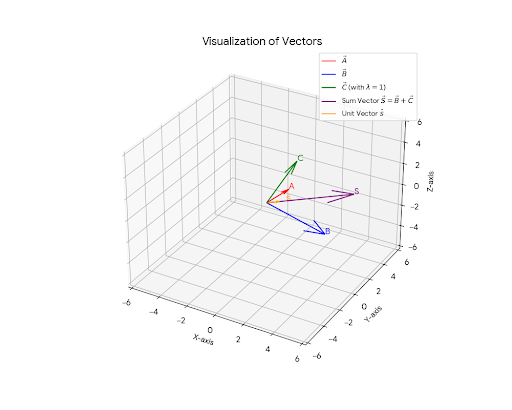
\includegraphics[width=0.8\linewidth]{figs/graph-1.png}
    \caption{}
    \label{fig:placeholder}
\end{figure}




\end{document}




\end{document}